\documentclass{article}
\author{Robbie Ellis \& Junseo Shin \& Daniel Rothstein}
\date{}
\title{Lab Notebook: Fourier Methods}

\usepackage{custom}
% use myrefs.bib for bibliography
\begin{document}

\maketitle
\tableofcontents
\pagebreak


\pagestyle{fancy}
\lhead{R. Ellis \& J. Shin \& D. Rothstein}
\rhead{Lab Notebook: Low Temperature Physics}
\chead{10/3/24}
% Day 1

\section*{Intro}
\addcontentsline{toc}{section}{Intro}

\paragraph{Low Temp 101}
Using log temp scale to measure superductivity, electron-phonon and electron-defect scattering phenomena using vacuums and cryogenics. 

\subsection{Samples}

\begin{itemize}
    \item Copper (Cu) Wire
    \begin{itemize}
        \item Diameter $D = 165 \pm \qty{10}{\micro m}$, Length $l = 482.0 \pm \qty{0.5}{cm}$: Area $A = \pi D^2/4$
        \item Bloch-G\"uneisen formula
        \begin{align} \label{eq:1} 
             [\rho(T) - \rho_0] = 4\rho_\Theta \qt(\frac{T}{\Theta})^5 \int_0^{\frac{\Theta}{T}} \frac{z^5 dz}{(e^z -1)(1 - e^z)}
        \end{align}
        where 
        \begin{align*}
            [\rho(T) - \rho_0] = \begin{cases}
                124.4  & T \ll \Theta \\
                \qt(\frac{T}{\Theta}) \rho_\Theta & T \gg \Theta
            \end{cases}
        \end{align*}    
        or for a free electron gas
        \begin{align*}
            [\rho(T) - \rho_0] = 497.6 \qt(\frac{T}{\Theta})^5 \rho_\Theta
        \end{align*}
    \end{itemize}
    \item Dysprosium (Dy) foil
    \begin{itemize}
        \item Width $w = (2.7 \pm 0.2)$ mm, Thickness $t = (0.11 \pm 0.01)$ mm, Length $l = (18.0 \pm 0.5)$ mm: Area $A = wt$
        \item Ferromagnetic ordering (spins align) below Curie Temp
        \item Phase transition to HCP (Hexagonal Close-Packed)
    \end{itemize}
    \item Niobium Titanium (NbTi) wire
    \begin{itemize}
        \item Diameter $D = 114 \pm 4$ $\mu$m, Length $l = 10.0 \pm 0.4$ cm: Area $A = \pi D^2/4$
        \item Superconducting transition temperature at $T_c = 9.50$ K \cite{manuel}
        \item Electrical resisivity $\rho \to 0$ at $T < T_c$
        \item Type II superconductor: Solenoid can generate $9$ T magnetic field at $4$ K
    \end{itemize}
    \item Lead (Pb) foil
    \begin{itemize}
        \item Width $w = 1.6 \pm 0.2$ mm, Thickness $t = 0.12 \pm 0.01$ mm, Length $l = 17.0 \pm 0.5$ mm: Area $A = wt$
        \item Superconducting (Type I) transition temperature at $T_c = 7.19$ K \cite{superlist}
        \item 
    \end{itemize}
\end{itemize}

\subsection{Measuring Resistivity}
\begin{figure}[ht]
    \centering
    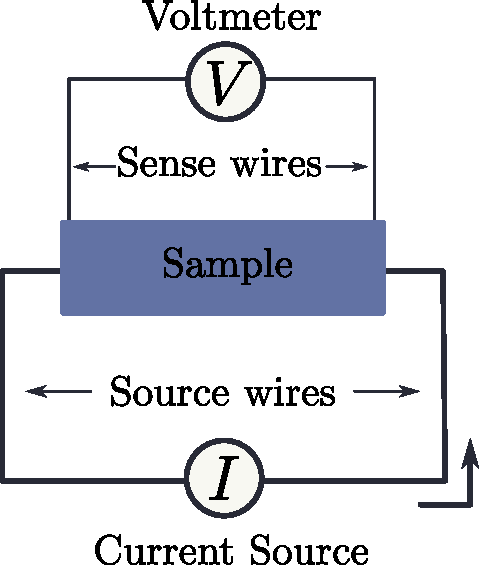
\includegraphics[width=0.4\textwidth]{4terma.pdf}
    \caption{Four-point measurement: 1 \& 4 are force leads, 2 \& 3 are sense leads.}
    \label{fig:thermometer}
\end{figure}
\begin{itemize}
    \item 4 terminal remote sensing: to reduce voltage drop from force leads
    \item Resistivity to resistance formula
    \begin{align*}
        \rho = R \frac{A}{l} = \frac{VA}{Il}
    \end{align*}
    where $I = 1$ mA for wire (Cu and NbTi) and $I = 10$ mA for foil (Dy and Pb)
    \item fractional error for Cu and NbTi
    \begin{align*}
        \frac{\delta p}{p} = \sqrt{\qt(2 \frac{\delta D}{D})^2 + \qt(\frac{\delta l}{l})^2 + \qt(\frac{\delta V}{V})^2 + \qt(\frac{\delta I}{I})^2}
    \end{align*}
    and for Dy and Pb
    \begin{align*}
        \frac{\delta p}{p} = \sqrt{\qt(\frac{\delta w}{w})^2 + \qt(\frac{\delta t}{t})^2 + \qt(\frac{\delta l}{l})^2 + \qt(\frac{\delta V}{V})^2 + \qt(\frac{\delta I}{I})^2}
    \end{align*}
\end{itemize}

\subsection{Measuring Temperature}
Using Chebyshev polynomial fit from Cernox manual to convert Resistance to temperature
\begin{align*}
    \log_{10} T = \sum_{i} a_i \cos(iw \log_{10} R) + b_i \sin(iw \log_{10} R)
\end{align*}

\newpage 
\begin{figure}[ht]
    \centering
    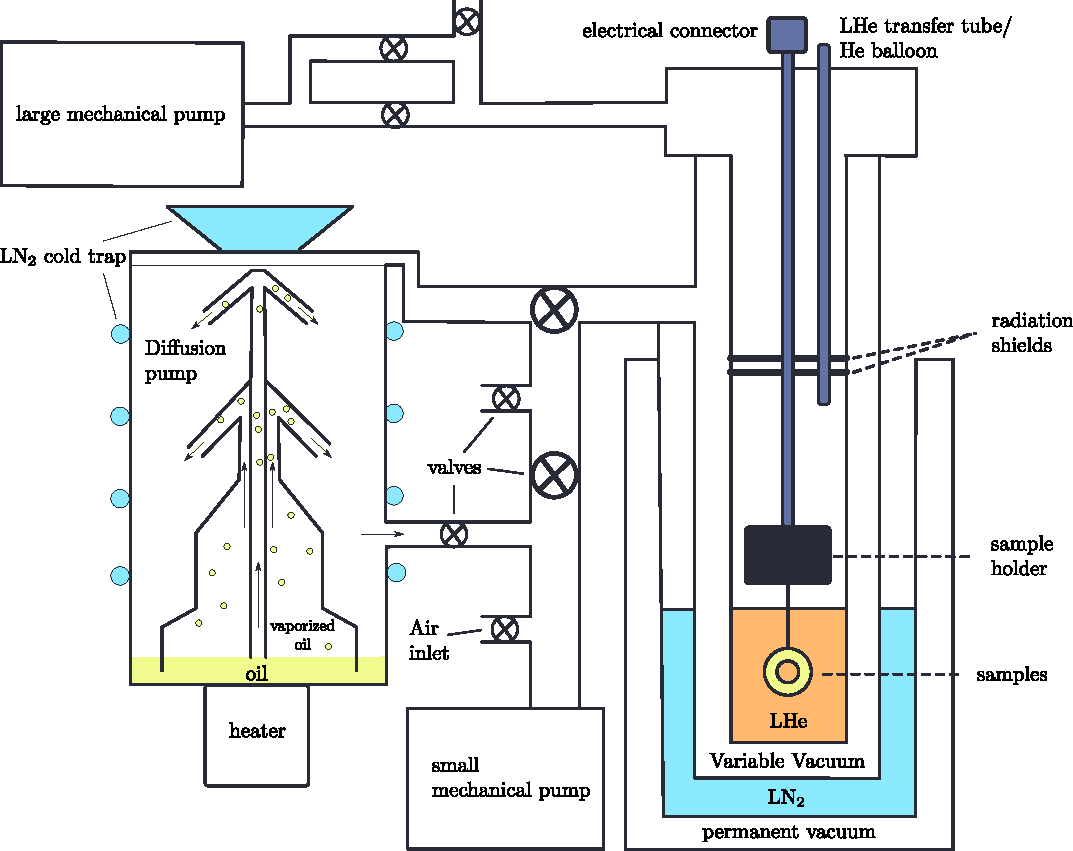
\includegraphics[width=0.7\textwidth]{apparatus.pdf}
    \caption{Main low temp apparatus: Drawn by Junseo! with help from Lab Manual}
    \label{fig:apparatus}
\end{figure}
\subsection{Cooling}
\begin{itemize}
    \item Cooling to 80 K
    \begin{itemize}
        \item Variable Vacuum $\to$ 5-10 Torr (5-10 mbar); Check Pressure with G1 (Pirani Gauge)
        \item Release V2 to $\downarrow$ P; V3 to $\uparrow$ P Until 5-10 Torr
        \item Fill LN$_2$ into OUTER DEWAR
        \item Wait roughly 4 hours to cool down to $\sim 80$ K, refilling LN$_2$ as needed
        \item Once we reach 80 K, let the sample warm back up to room temp
    \end{itemize}

\end{itemize}



\chead{10/8/24}
\section{Data \& Analysis}
\subsection{DATA COLLECTION DAY 1:}

\paragraph{LAB CHART CONFIG}
\begin{itemize}
    \item Multiscan: Time between cycles $= 30$ s; Number of cycles $= 4000 \implies$ Total time $120000$ s
    \item Timing: 200 ms Integration period; Range $-100mV \to 100mV$ 
    \item Variable Vacuum: 220; 215; 205
\end{itemize}

\paragraph{Notes}
\begin{itemize}
    \item We were able to cool down the sample to 80 K in preparation for the next 
    experiment to cool the samples down to 4 K.
    \item Using the Multimeters and the lookup chart, we can quickly convert the voltage readings to temperature. But at room temperature,
    a voltage of $4.926\text{mV}$, corresponded to a temperature of around $278\text{K}$ based off the manufacturer calibration settings which is quite cold.
    For room temp ($\sim 293.0K$) the predicted measured voltage is around $4.743\text{mV}$. So there must be calibrations
    made to a reading to correct the temperature from the $15$ K offset.
\end{itemize}

\newpage
\chead{10/17/24}
\subsection{DATA COLLECTION DAY 2}
\paragraph{LAB CHART CONFIG}
\begin{itemize}
    \item Multi Scan: 30s Time between cycles; 4000 cycles $\implies$ 120,000 s
    \item Timing: 200 ms Integration period; Range $-100mV \to 100mV$ 
    \item Variable Vacuum: $\to 80$ K, 4.57 Torr; $\to 4K$, 0.39 Torr; Cool down to room temp $5.67$ Torr at the end.
\end{itemize}

\subsection*{Cooling to 4 K}
\begin{itemize}
    \item Bringing Variable Vacuum to $< \qty{e-4}{Torr}$:
    \begin{itemize}
        \item open V2
        \item open v4
        \item small pump on
        \item Heater + fan + LN$_2$ on
        \item wait 20 minutes to wamr up
        \item open v1
        \item close v2
    \end{itemize} 
    \item Adding liquid helium LHe (it is fragile in air):
    \begin{itemize}
        \item Fill chamber with Helium gas (it comes out of rubber stop)
        \item What the voltage wil read at 4.2 K: $400 \Omega \to 4$ mV
        \item Why do we take out the helium? As we take out the helium, 
        \item Superfluid transition below $20 K \to 4K$ happens really fast.
        \item Bfore adding LHe, remove rubber stop to vent inner dewar to 1 atm (if we don't do this, a sudden pressure build up will explode the glass)
        \item Change current to 10 $\mu$ A for less than 40 K
        \item Change current to 1 $\mu$ A for less than $2.57$ K
    \end{itemize}
    \item Measuring helium vapor Pressure
    \begin{itemize}
        \item Replace balloon with tube to analog pressure gauge
        \item Slowly release V7 (with rubber stopper in and V8 closed)
        \item to reduce pressure when V7 is fully open, slowly open V6
        \item Record Pressure and Temp at equilibrium
    \end{itemize}
\end{itemize}
\paragraph{Notes}
\begin{itemize}
    \item Some obstacles in cooling down to 4 K:
    \begin{itemize}
        \item The diffusion pump was left on since the last lab group, which led to some inconsistencies in getting the
        inner dewar to a low enough vacuum pressure before starting the liquid cool down.
        \item We weren't able to get full data down to $\sim 1$ K as we ran out of LHe. 
        Although we were able to get a few data points for the vapor pressure vs temperature. 
        \item Furthermore, we were unable to get precise measurements for slow temperature change via raising the samples above the LHe bath.
    \end{itemize}
\end{itemize}

\newpage
\chead{10/22-29/24}
\subsection{Data Analysis}
\begin{itemize}
    \item Resistivity Error Analysis: Example for Copper Wire
    \begin{align*}
        \frac{\delta p}{p} &= \sqrt{\qt(2 \frac{\delta D}{D})^2 + \qt(\frac{\delta l}{l})^2 + \qt(\frac{\delta V}{V})^2 + \qt(\frac{\delta I}{I})^2} \\
        &= \sqrt{\qt(2 \frac{10}{165})^2 + \qt(\frac{0.5}{482})^2} = 0.121 \implies 10 \%
    \end{align*}
    with negligible error in $V$ and $I$ since they are measured with high precision.
    % table of fractional uncertatainty delta p/p for each sample Dy Pb NbTi Cu
    \begin{table}[ht]
        \centering
        \begin{tabular}{|c|c|}
            \hline
            Sample & $\delta p/p$ \\
            \hline
            Cu & 10 \% \\
            \hline
            NbTi & 8 \% \\
            \hline
            Pb & 20 \% \\
            \hline
            DY & 10 \% \\
            \hline
        \end{tabular}
        \caption{Fractional uncertainty in resistivity for each sample}
        \label{tab:resistivity}
    \end{table}
    \item Resistance $\to$ Temperature conversion using Chebyshev polynomial fit python code:
    % python code for fitting chebyshev polynomial
    \begin{lstlisting}[language=Python]
    import numpy as np

    def temp_K(ohm):
        a = [.8992, -.5026, .1524, -.306, .3517, -.204, 0.03868, 0.01532, -0.006606]
        b = [0, -1.226, .5757, -.3768, .1169, .09066, -.09729, .03033, -.001984]
        w = 2.299
        logT = 0;
        for i in range(0, len(a)):
        logT += a[i] * np.cos(i * np.log10(ohm) * w) + b[i] * np.sin(i * np.log10(ohm) * w)
        return 10**logT
    \end{lstlisting}
    e.g. \texttt{print(temp\_K(1023.57))} prints out \texttt{1.19937} which matches the expected value from the lookup table.

    \subsection*{Preliminary Data Analysis}
    \item From log resistivity vs temperature, we can find the critical temperature $T_c$ for each sample: $\sim 10$ K which is visually close to the expected values.
    \begin{figure}[ht]
        \centering
        \begin{tabular}{cc}
            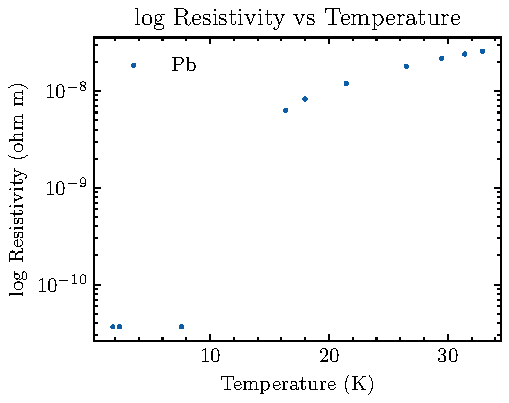
\includegraphics[width=0.4\textwidth]{pb_resistivity.pdf} & 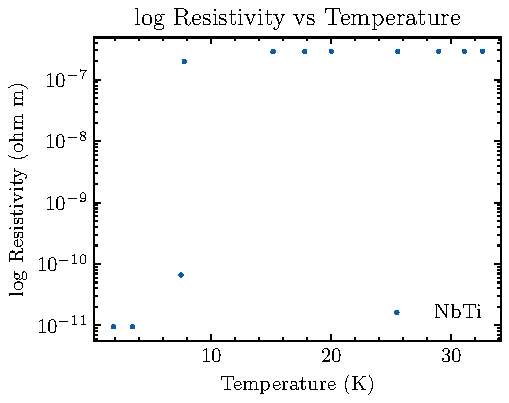
\includegraphics[width=0.4\textwidth]{nbti_resistivity.pdf} 
        \end{tabular}
        \caption{log Resistivity vs Temperature for finding critical temperature $T_c$}
    \end{figure}

    \newpage
    \item Vapor Pressure Temperature vs Voltage Temperature readings
    \begin{figure}[ht]
        \centering
        \begin{tabular}{cc}
            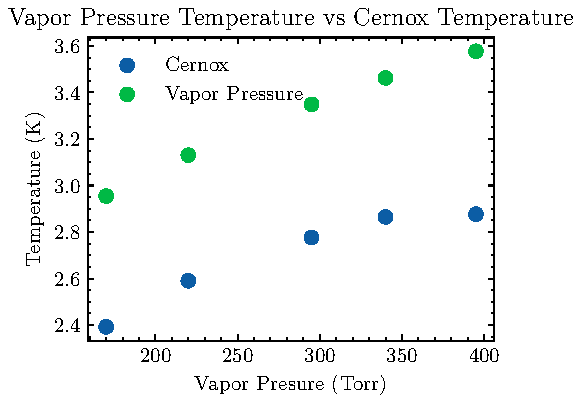
\includegraphics[width=0.45\textwidth]{cernox_vs_vapor.pdf}
        \end{tabular}
        \caption{Cernox comes from Voltage reading to Temperature, while Vapor Pressure comes from analog pressure gauge}
    \end{figure}
    
    \item RRR Calculation
    \begin{table}[ht]
        \centering
        \begin{tabular}{|c|c|c|c|}
        \hline
        Material & $\rho_{0}$ $(\text{n} \Omega \cdot \text{m})$ & $\rho_{293}$ $(\text{n} \Omega \cdot \text{m})$ & RRR  \\ 
        \hline
        NbTi & 298 & 356 & $1.19 \pm 0.14$ \\
        \hline
        Cu & 0.135 & 17.0 & $126 \pm 22$ \\
        \hline
        Dy & 62.7 & $1.13 \times 10^{3}$ & $18.8 \pm 3.3$\\
        \hline
        \end{tabular}
    \end{table}

    \item Bloch-G\"uneisen Formula Fit for Cu wire using numerical integration:
    \begin{figure}[ht]
        \centering
        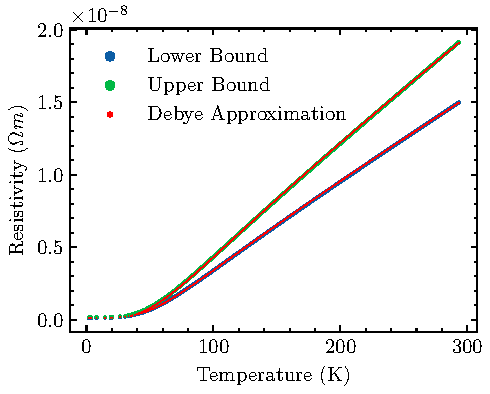
\includegraphics[width=0.45\textwidth]{resistivity_temp_cu.pdf}
        \caption{Bloch-G\"uneisen Formula Fit for Cu wire}
    \end{figure}

    We are unsure why the lower and upper bounds have such a large discrepancy, but the fit is quite reasonable for the data.

    \newpage
    \item Resistivity vs Temperature graphs for paper
    \begin{figure}[ht]
        \centering
        \begin{tabular}{cc}
            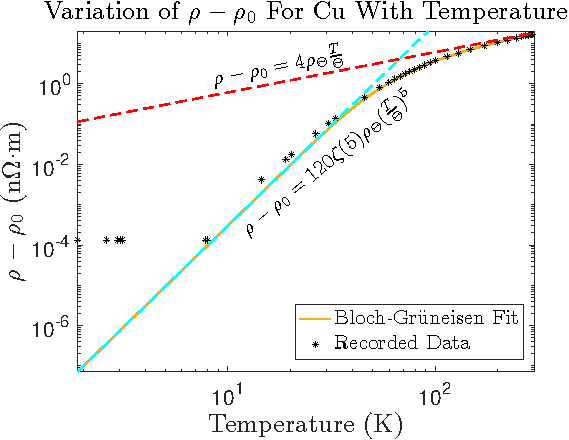
\includegraphics[width=0.45\textwidth]{cu_final.pdf} & 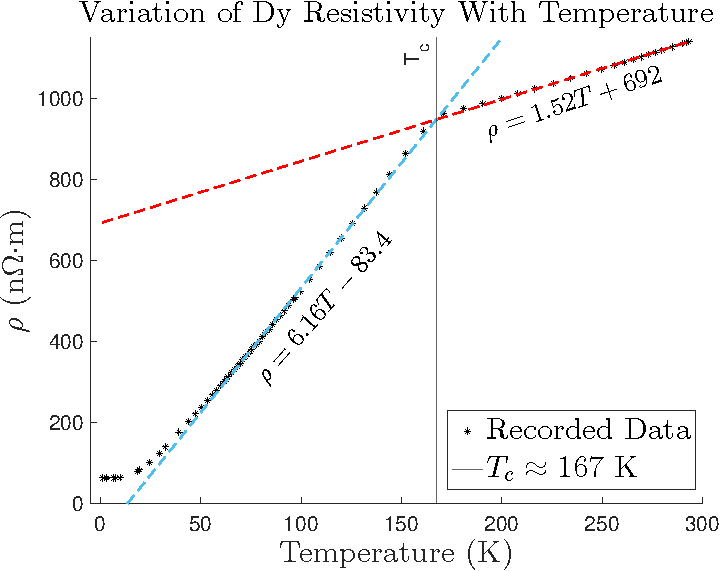
\includegraphics[width=0.45\textwidth]{dy_final.pdf} \\
            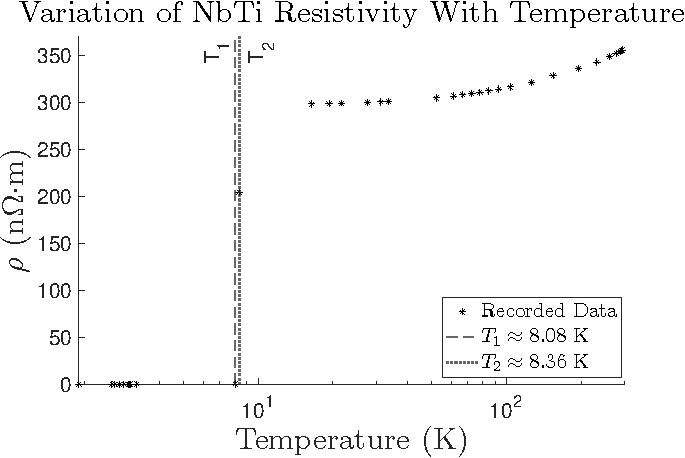
\includegraphics[width=0.45\textwidth]{nbti_final.pdf} & 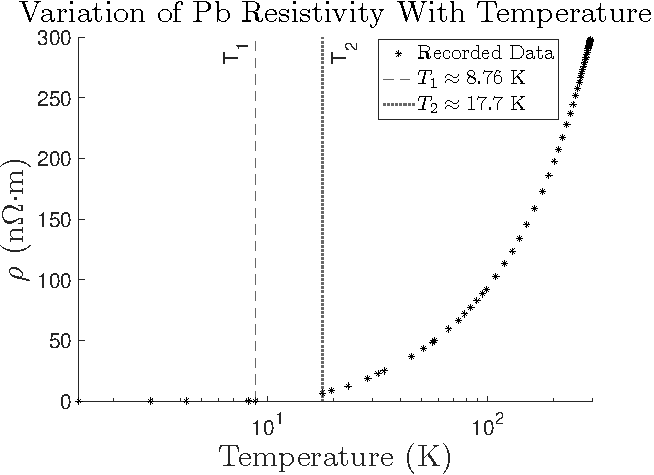
\includegraphics[width=0.45\textwidth]{pb_final.pdf} 
        \end{tabular}
        \caption{Resistivity vs Temperature for different materials}
    \end{figure}
\end{itemize}

\paragraph{Notes}
\begin{itemize}
    \item We were able to get the data for the resistivity vs temperature for all the samples, and we were able to get the RRR values for each sample.
    \item Upon further analysis, we had to account for the offset in the temperature reading for both high and low temperatures i.e. we sclaed the resistance by a factor of 0.9665 to get a slightly more accurate temperature reading.
    \item The RRR make sense for the samples: Cu has the highest RRR as it is a good conductor vs NbTi which only gets low resistivity after it becomes superconducting.
\end{itemize}

\bibliography{myrefs}
\bibliographystyle{plain}
\end{document}